\chapter{Sample Performance Metrics}

In this section, we present the results of 1 pair of nodes which are furthest apart in the simulation for the three formations. There are 36 nodes in the simulation.

\newgeometry{margin=1in,lmargin=1.25in,footskip=\chapterfootskip, includehead, includefoot}
%\thispagestyle{lscaped}
%\pagestyle{lscaped}
\thispagestyle{lscapedplain}

\begin{landscape}
\begin{figure}
\centering
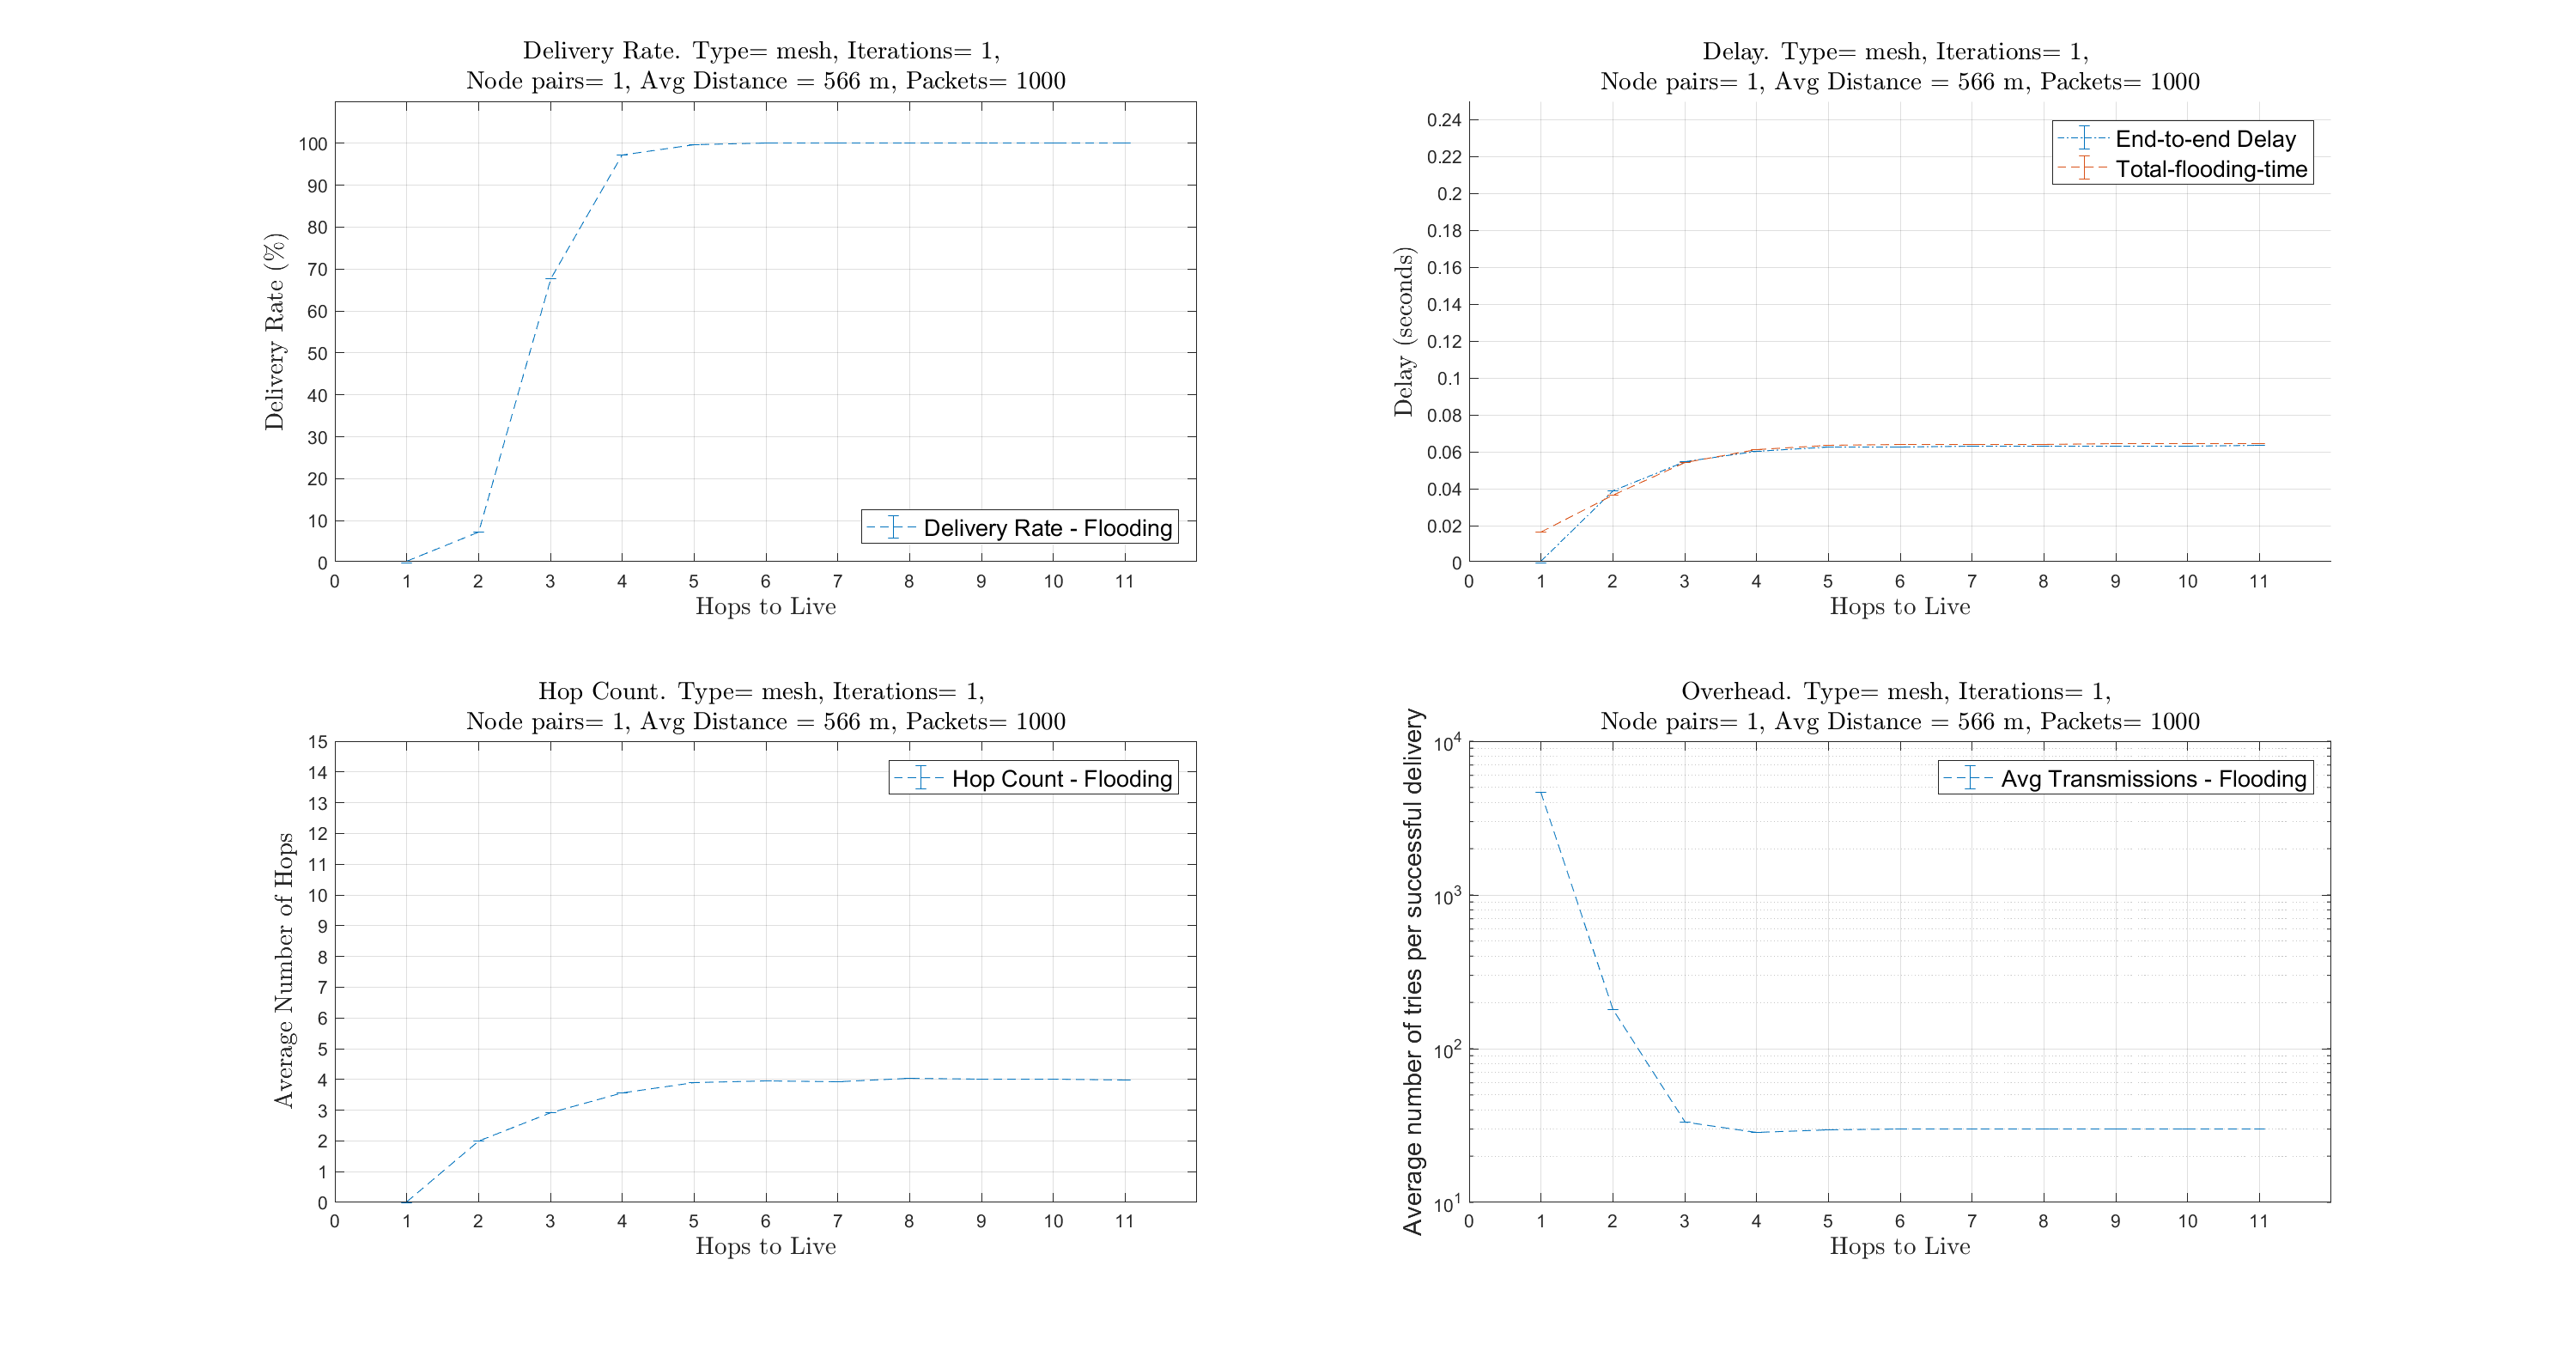
\includegraphics[width=1\textwidth]{ncsuthesis-0.6/Appendix-A/figs/flood_mesh}
\caption{Delivery ratio, end-to-end delay, hops and overhead for flooding algorithm in a 2 dimensional formation of UAVs.}
\label{fig:flood_mesh}
\end{figure}
\end{landscape}

\thispagestyle{lscapedplain}
\begin{landscape}
\begin{figure}
\centering
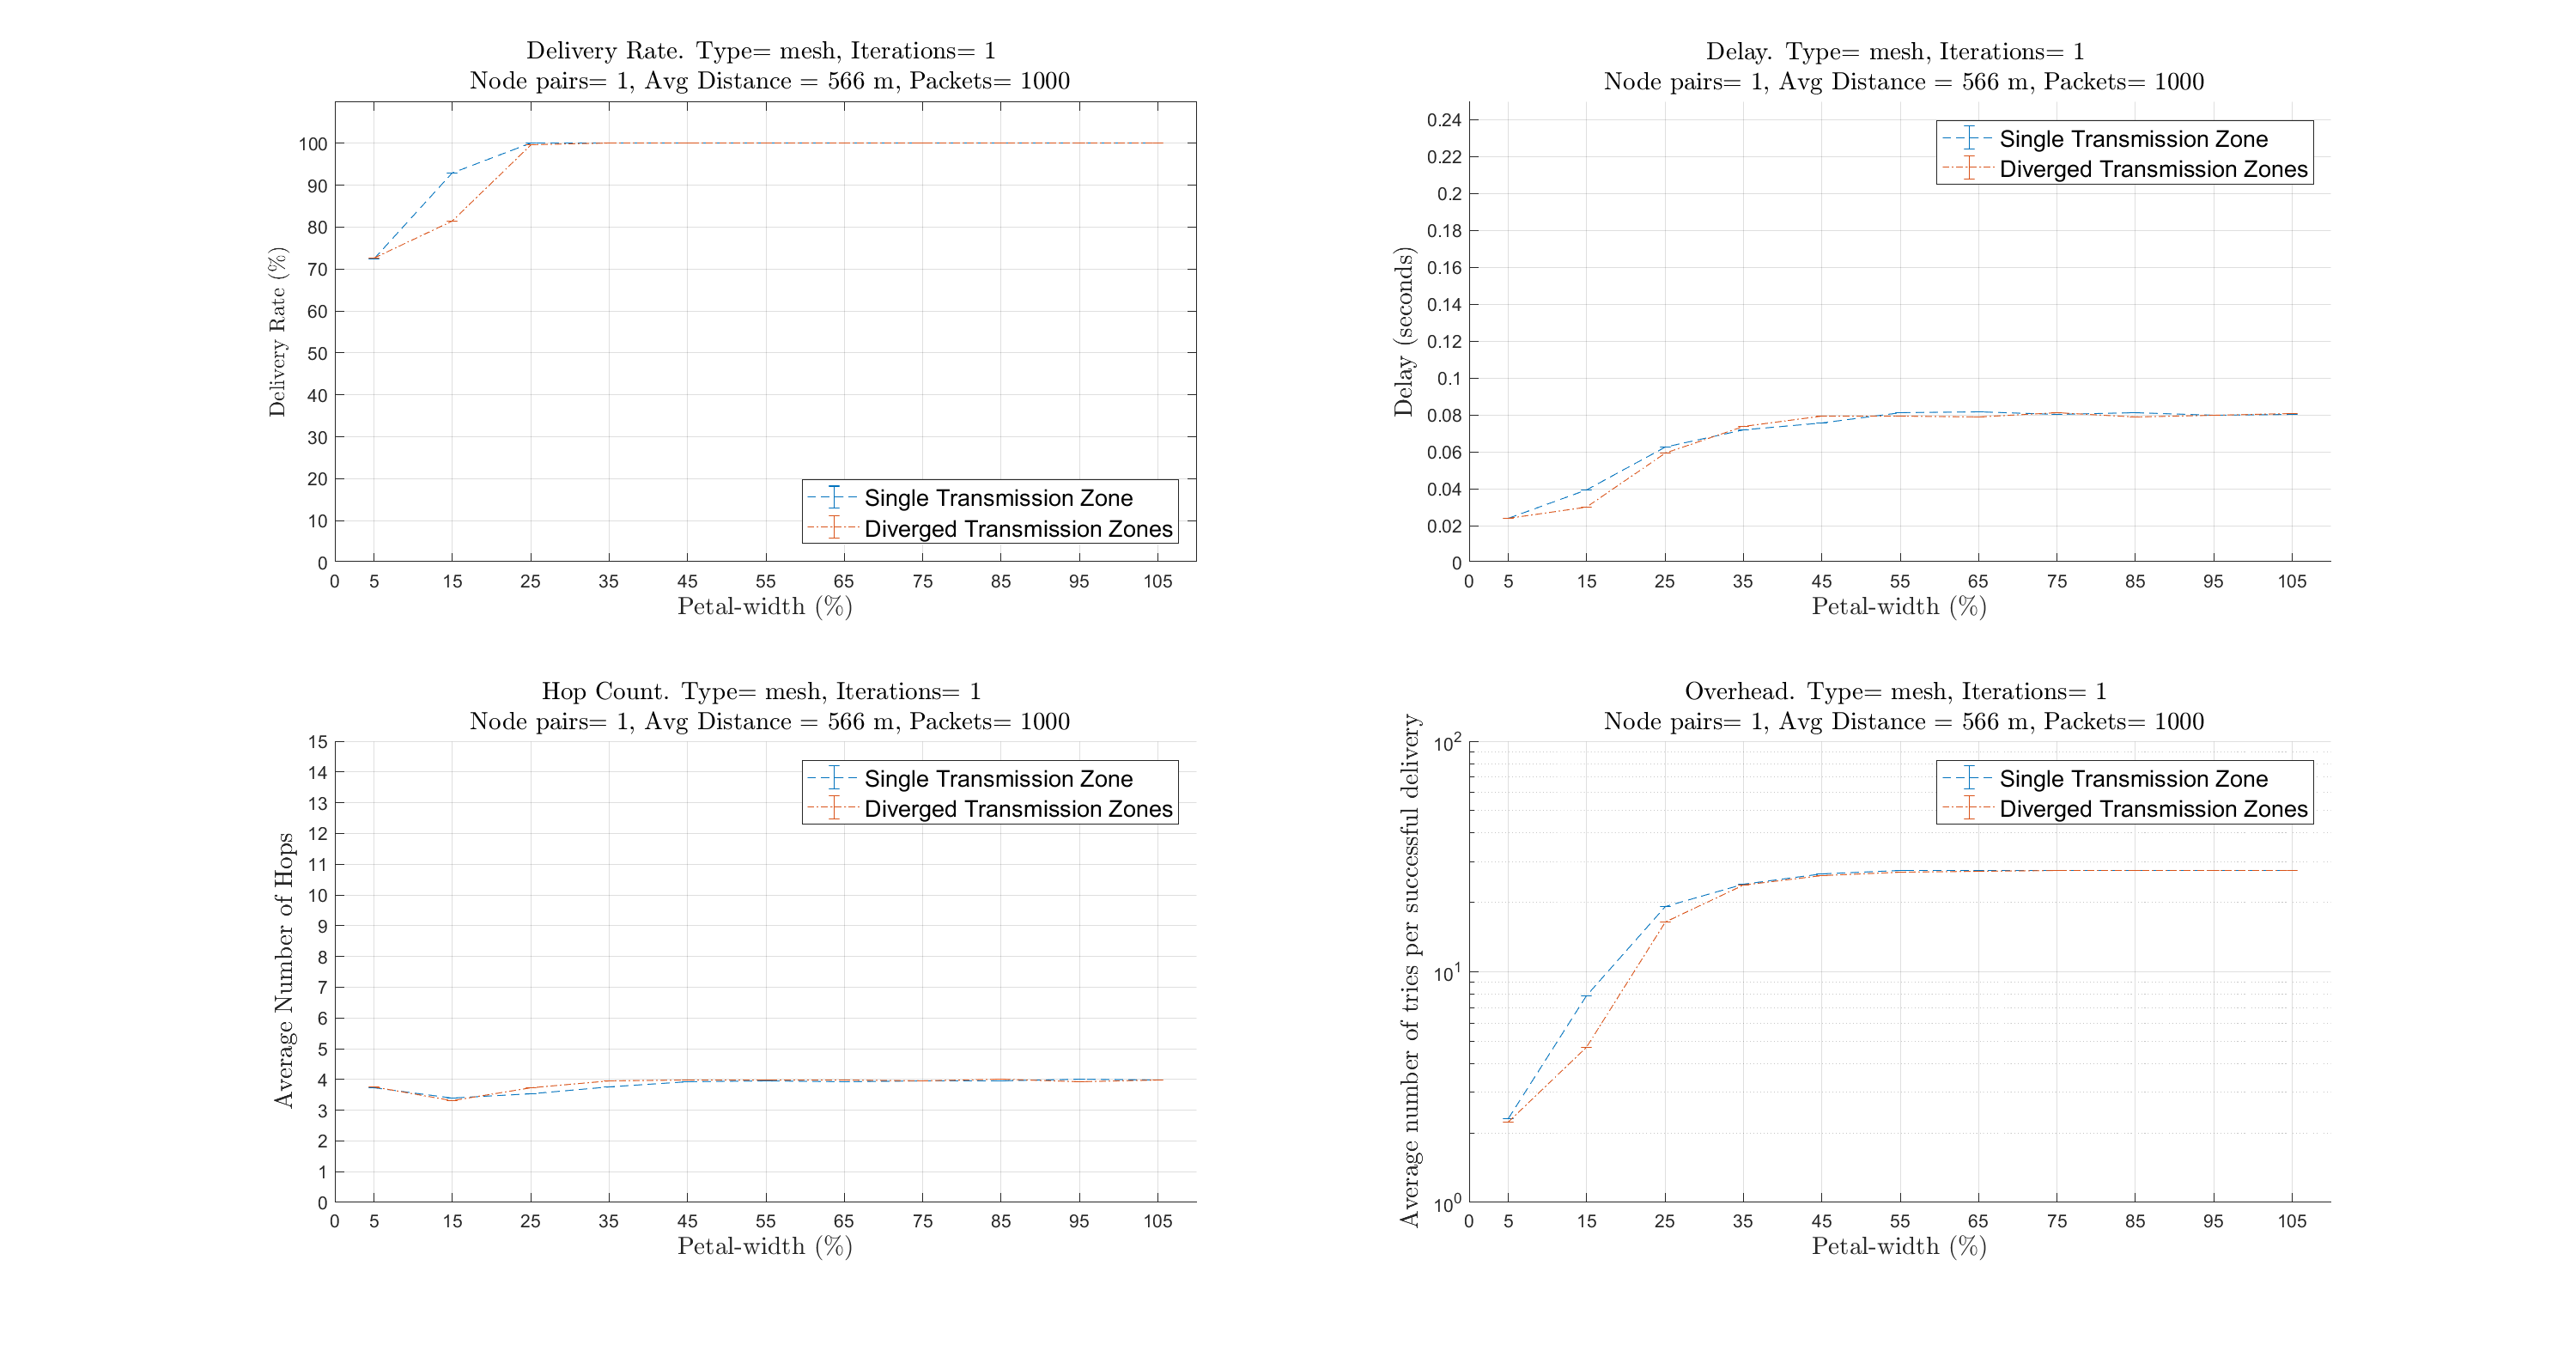
\includegraphics[width=1\textwidth]{ncsuthesis-0.6/Appendix-A/figs/petal_mesh.png}
\caption{Delivery ratio, end-to-end delay, hops and overhead for petal routing in a 2 dimensional formation of UAVs.}
\label{fig:petal_mesh}
\end{figure}
\end{landscape}

\thispagestyle{lscapedplain}
\begin{landscape}
\begin{figure}
\centering
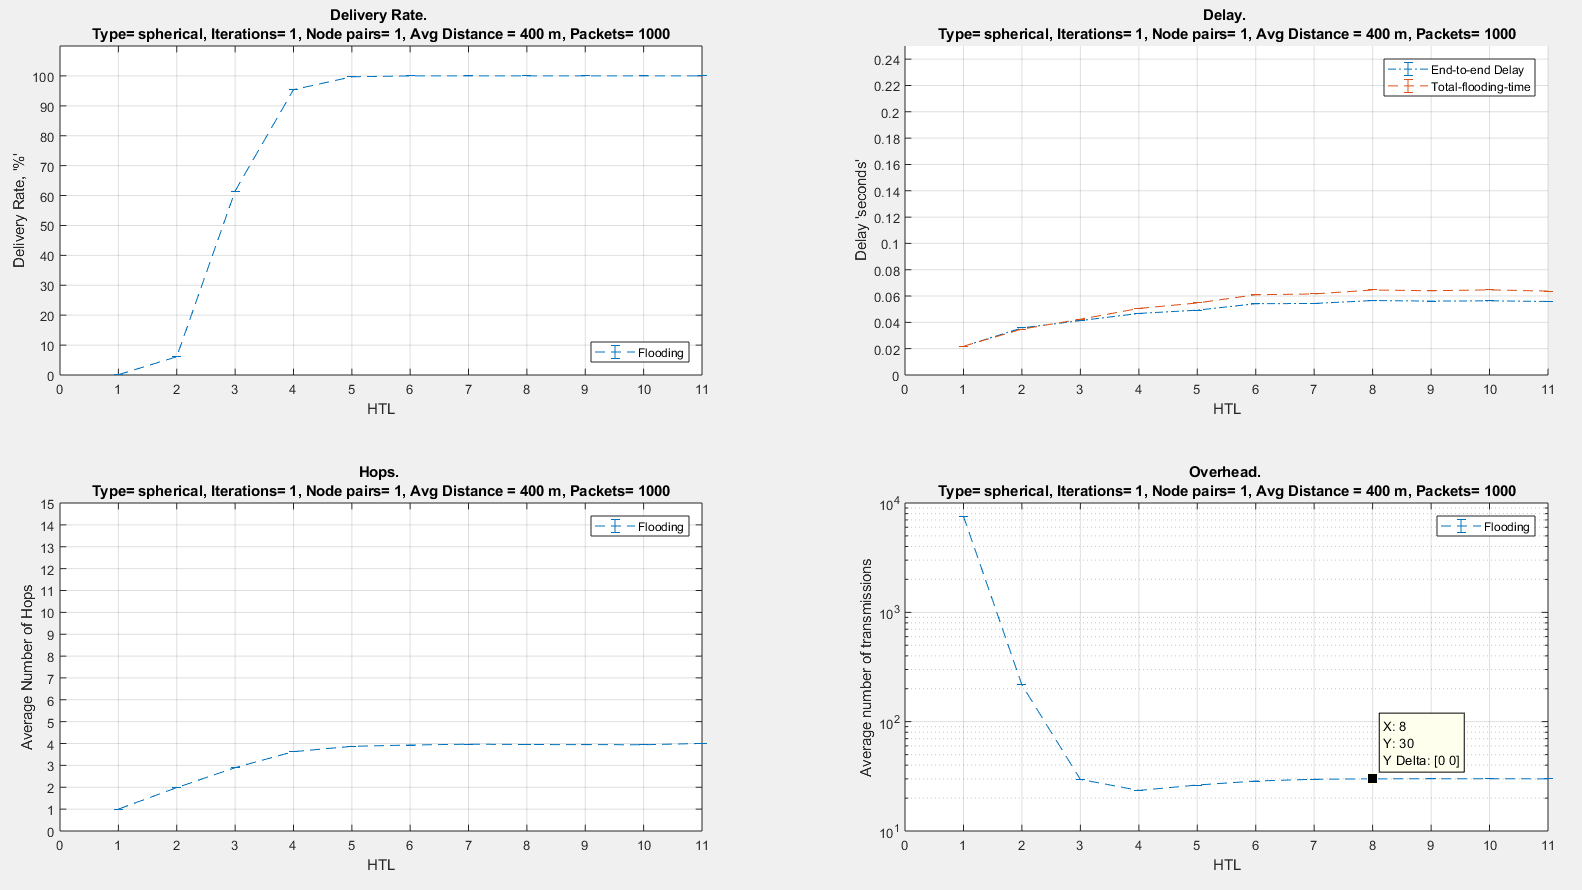
\includegraphics[width=1\textwidth]{ncsuthesis-0.6/Appendix-A/figs/flood_spherical.png}
%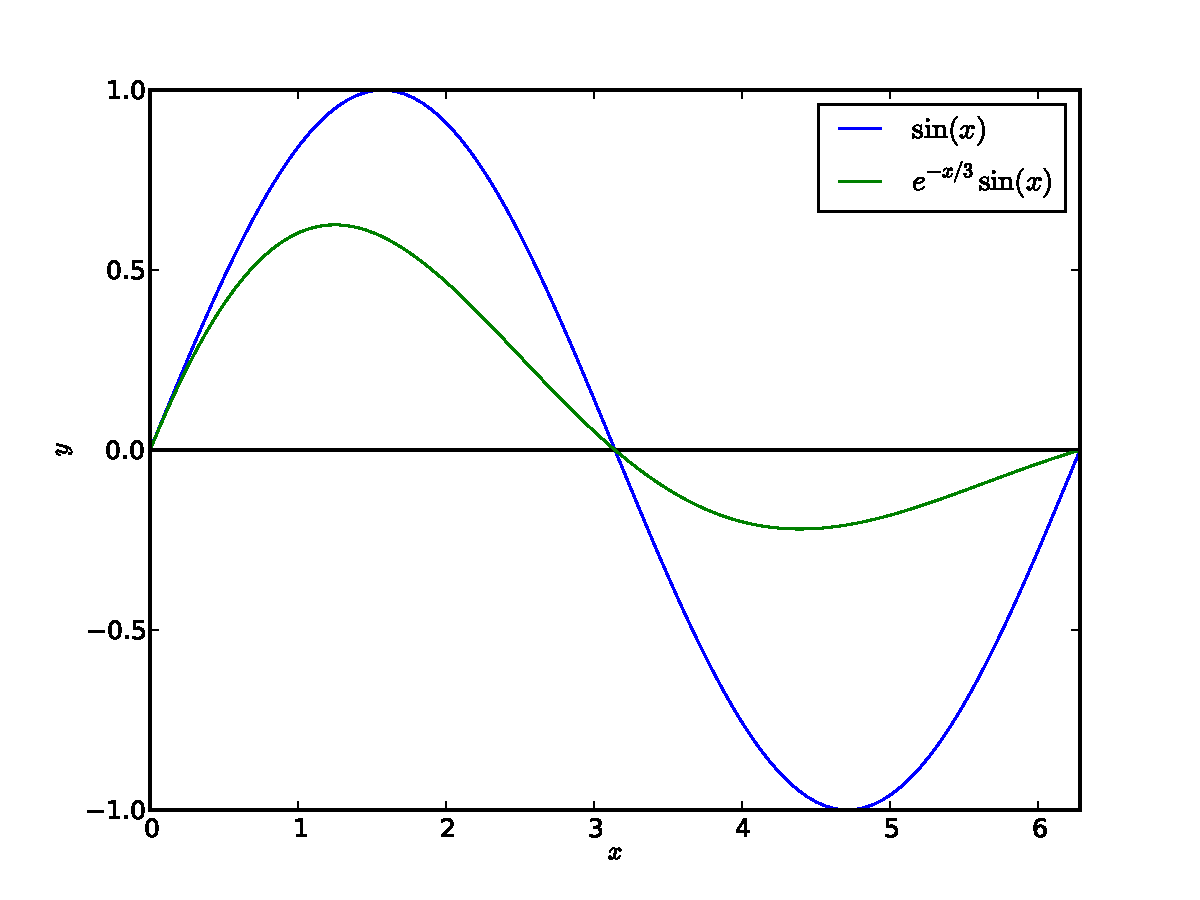
\includegraphics[height=\textwidth]{Chapter-2/figs/sine}
\caption{Delivery ratio, end-to-end delay, hops and overhead for flooding algorithm in a spherical arrangement of UAVs. }
\label{fig:flood_spherical}
\end{figure}
\end{landscape}

\thispagestyle{lscapedplain}
\begin{landscape}
\begin{figure}
\centering
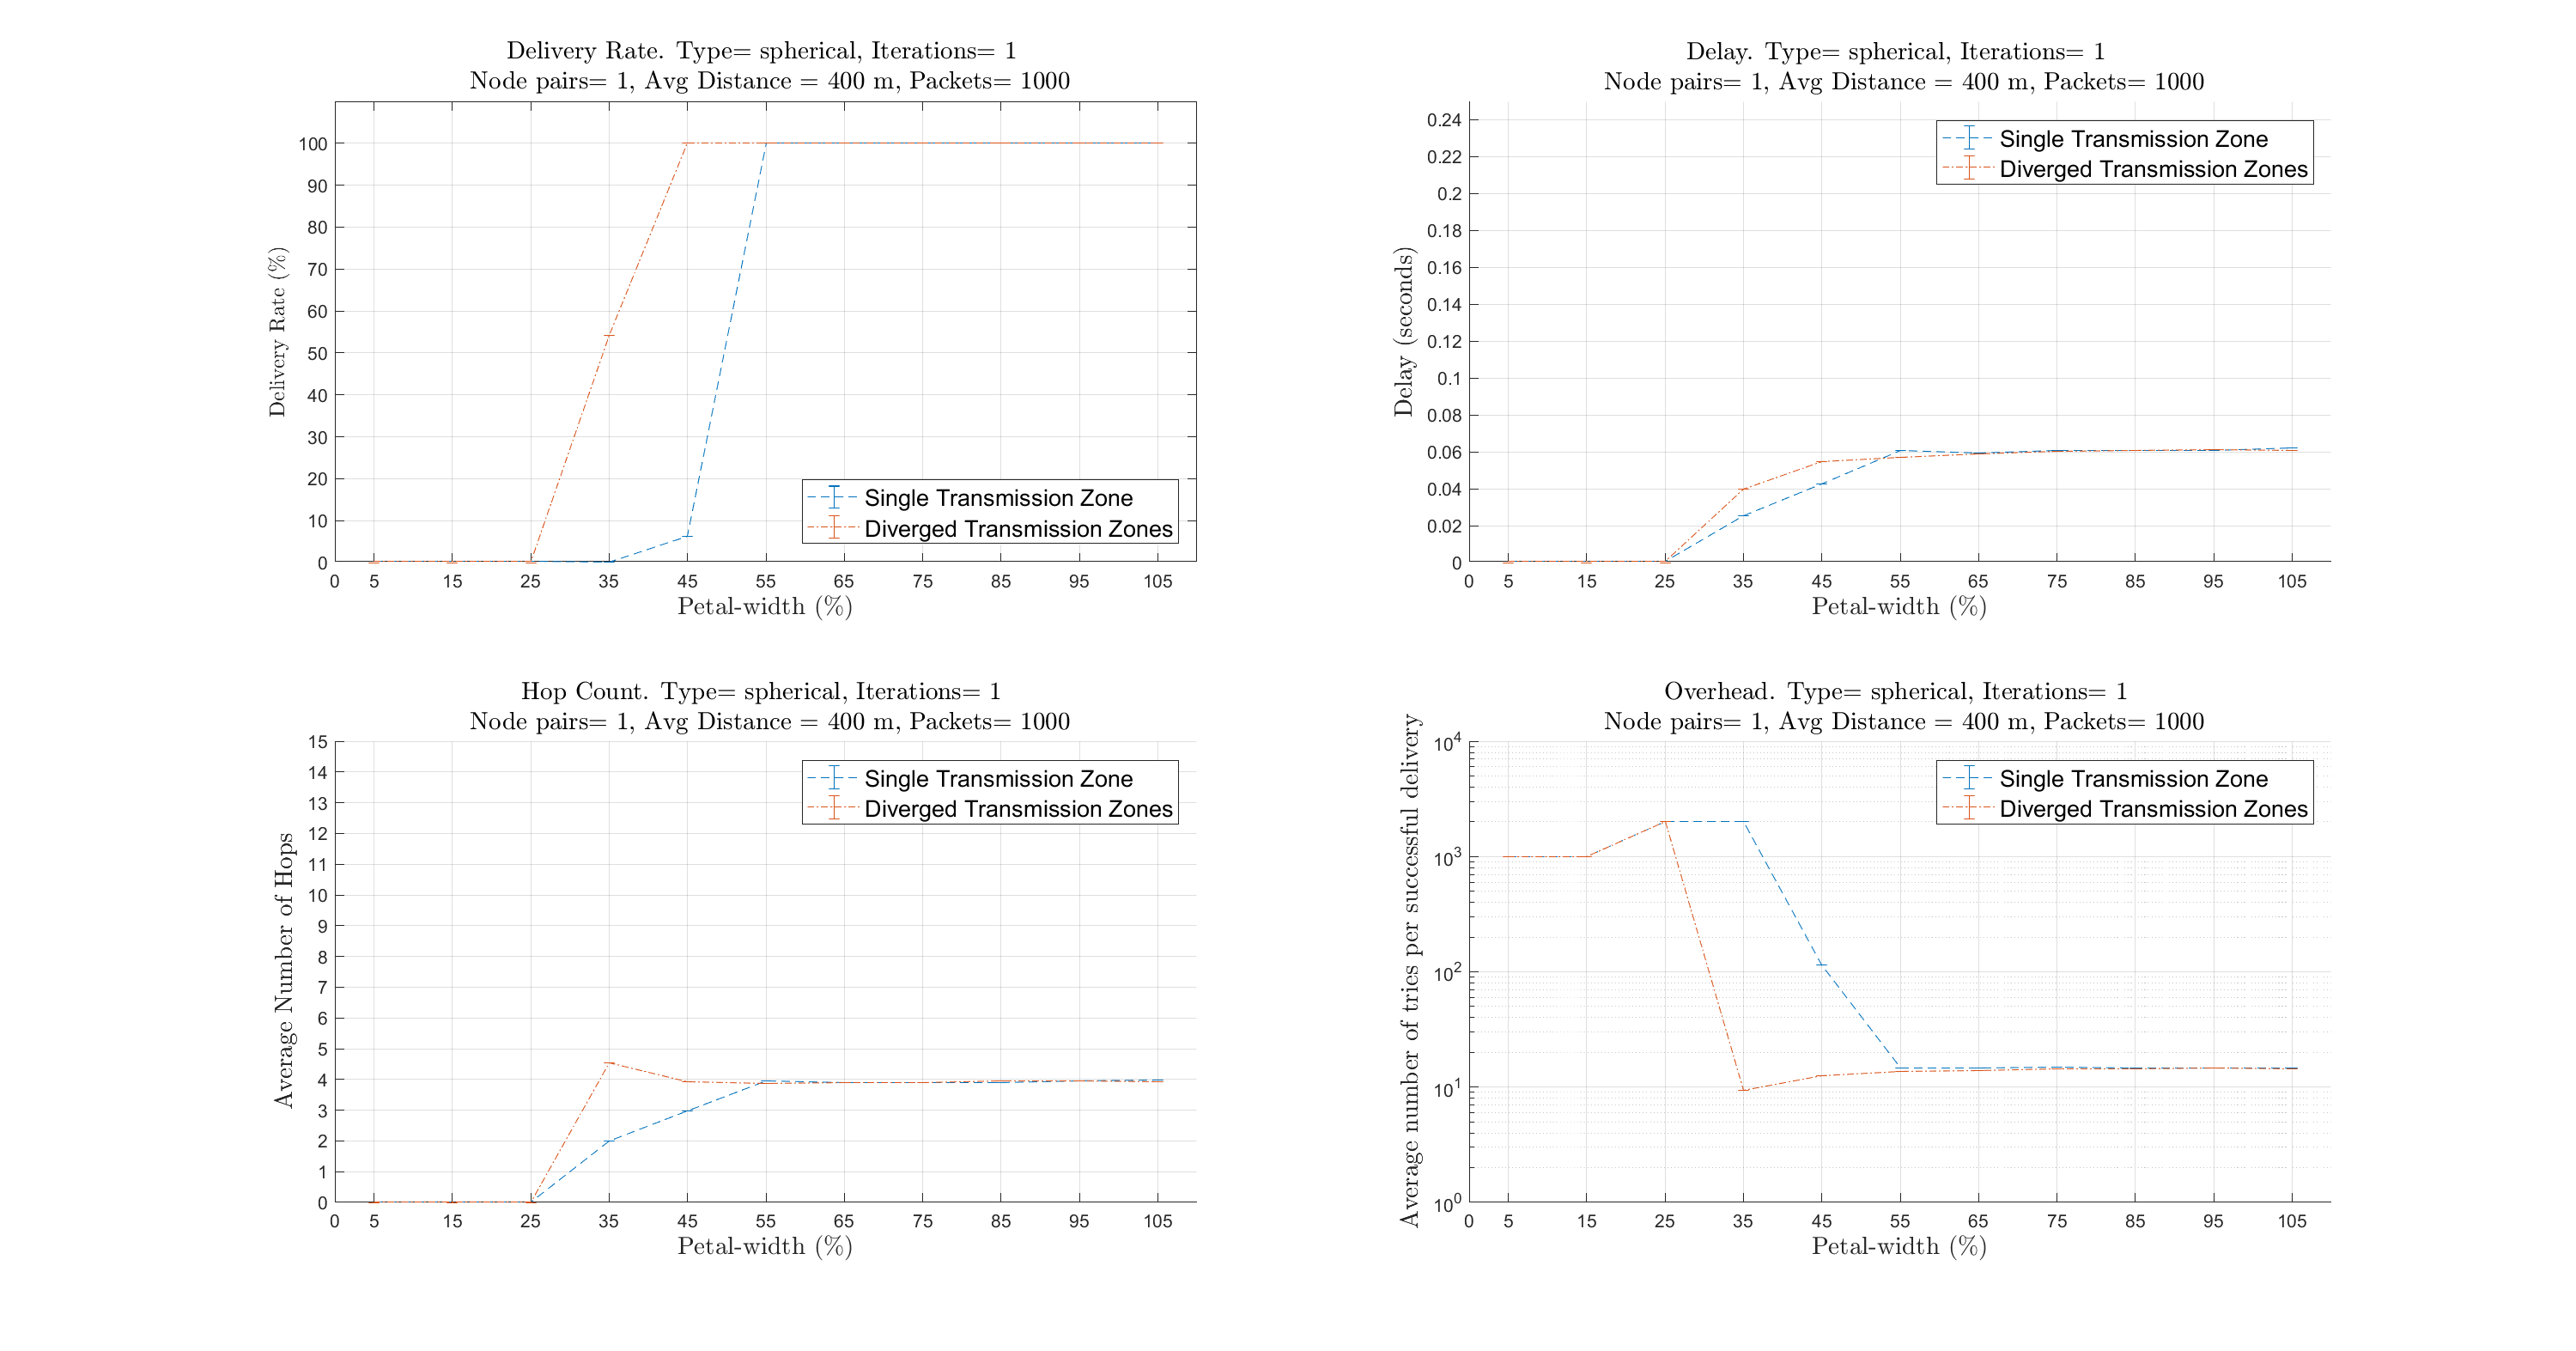
\includegraphics[width=1\textwidth]{ncsuthesis-0.6/Appendix-A/figs/petal_spherical.png}
%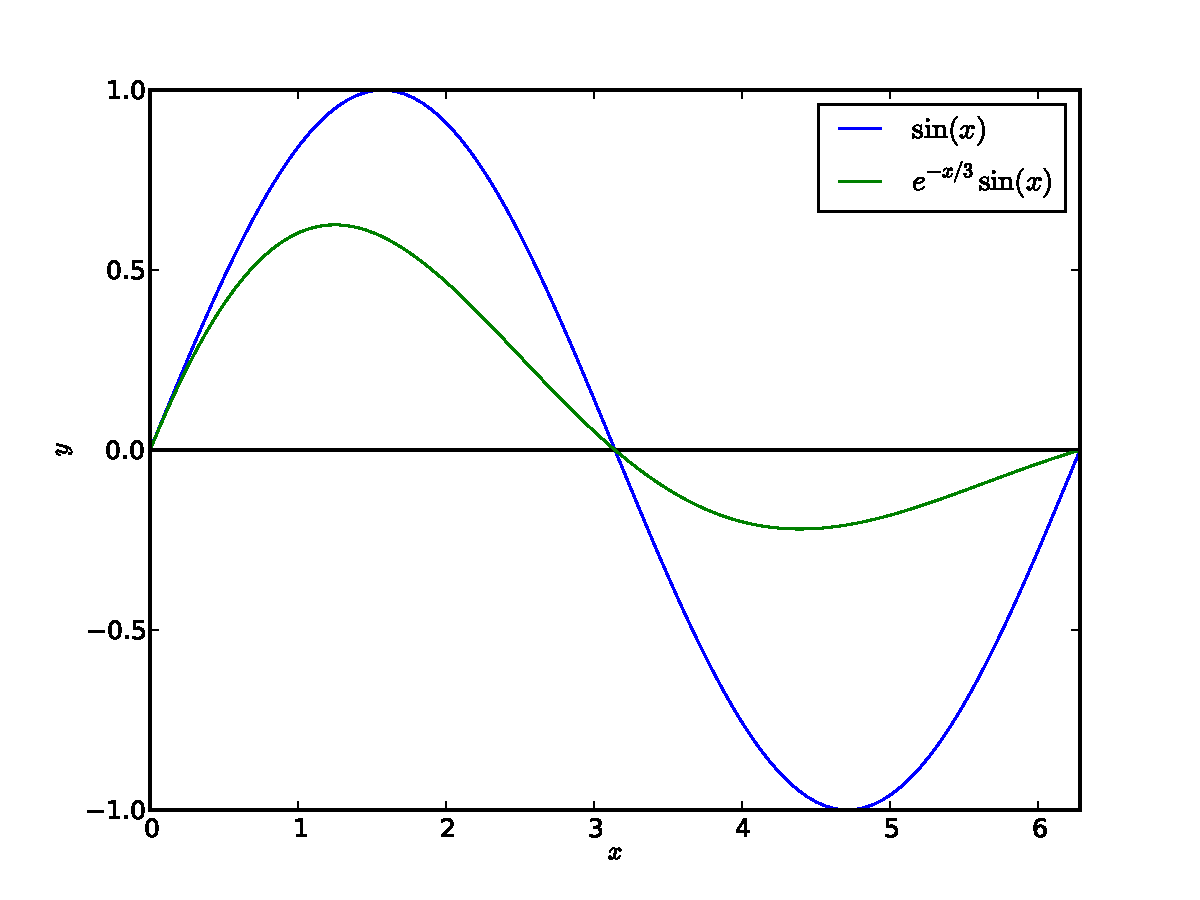
\includegraphics[height=\textwidth]{Chapter-2/figs/sine}
\caption{Delivery ratio, end-to-end delay, hops and overhead for petal routing in a spherical arrangement of UAVs.}
\label{fig:petal_spherical}
\end{figure}
\end{landscape}

\thispagestyle{lscapedplain}
\begin{landscape}
\begin{figure}
\centering
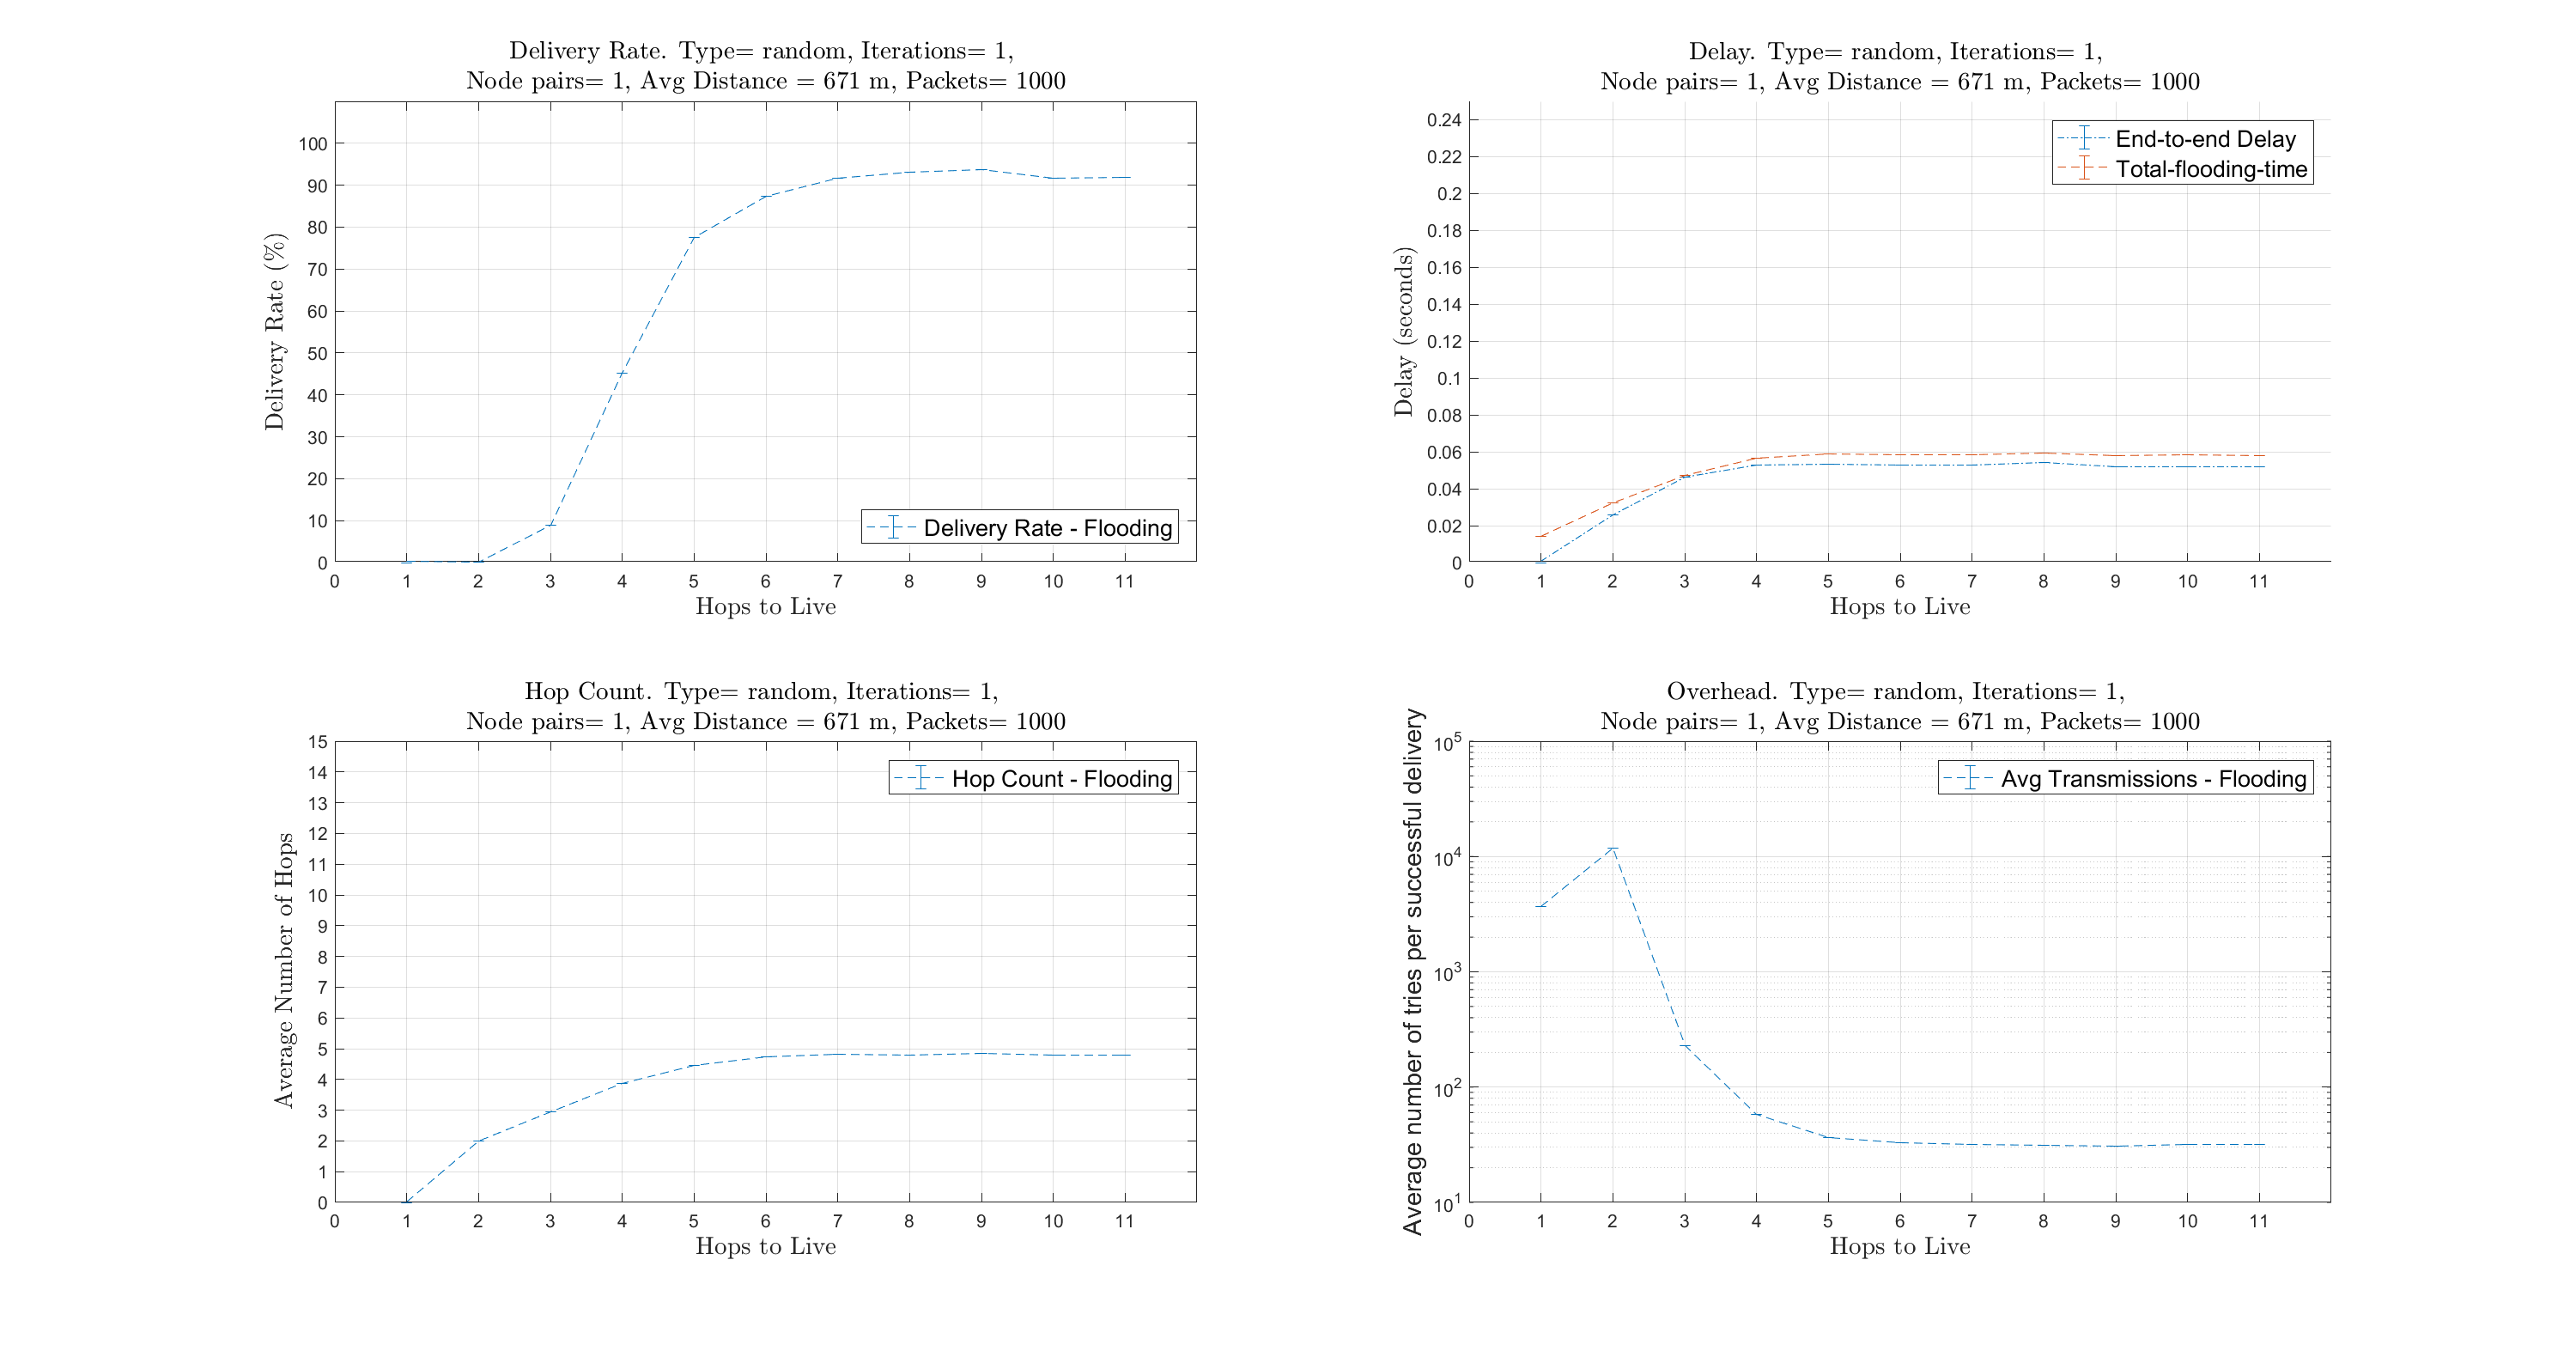
\includegraphics[width=1\textwidth]{ncsuthesis-0.6/Appendix-A/figs/flood_random.png}
\caption{Delivery ratio, end-to-end delay, hops and overhead for flooding algorithm in a random distribution of UAVs.}
\label{fig:flood_random}
\end{figure}
\end{landscape}

\thispagestyle{lscapedplain}
\begin{landscape}
\begin{figure}
\centering
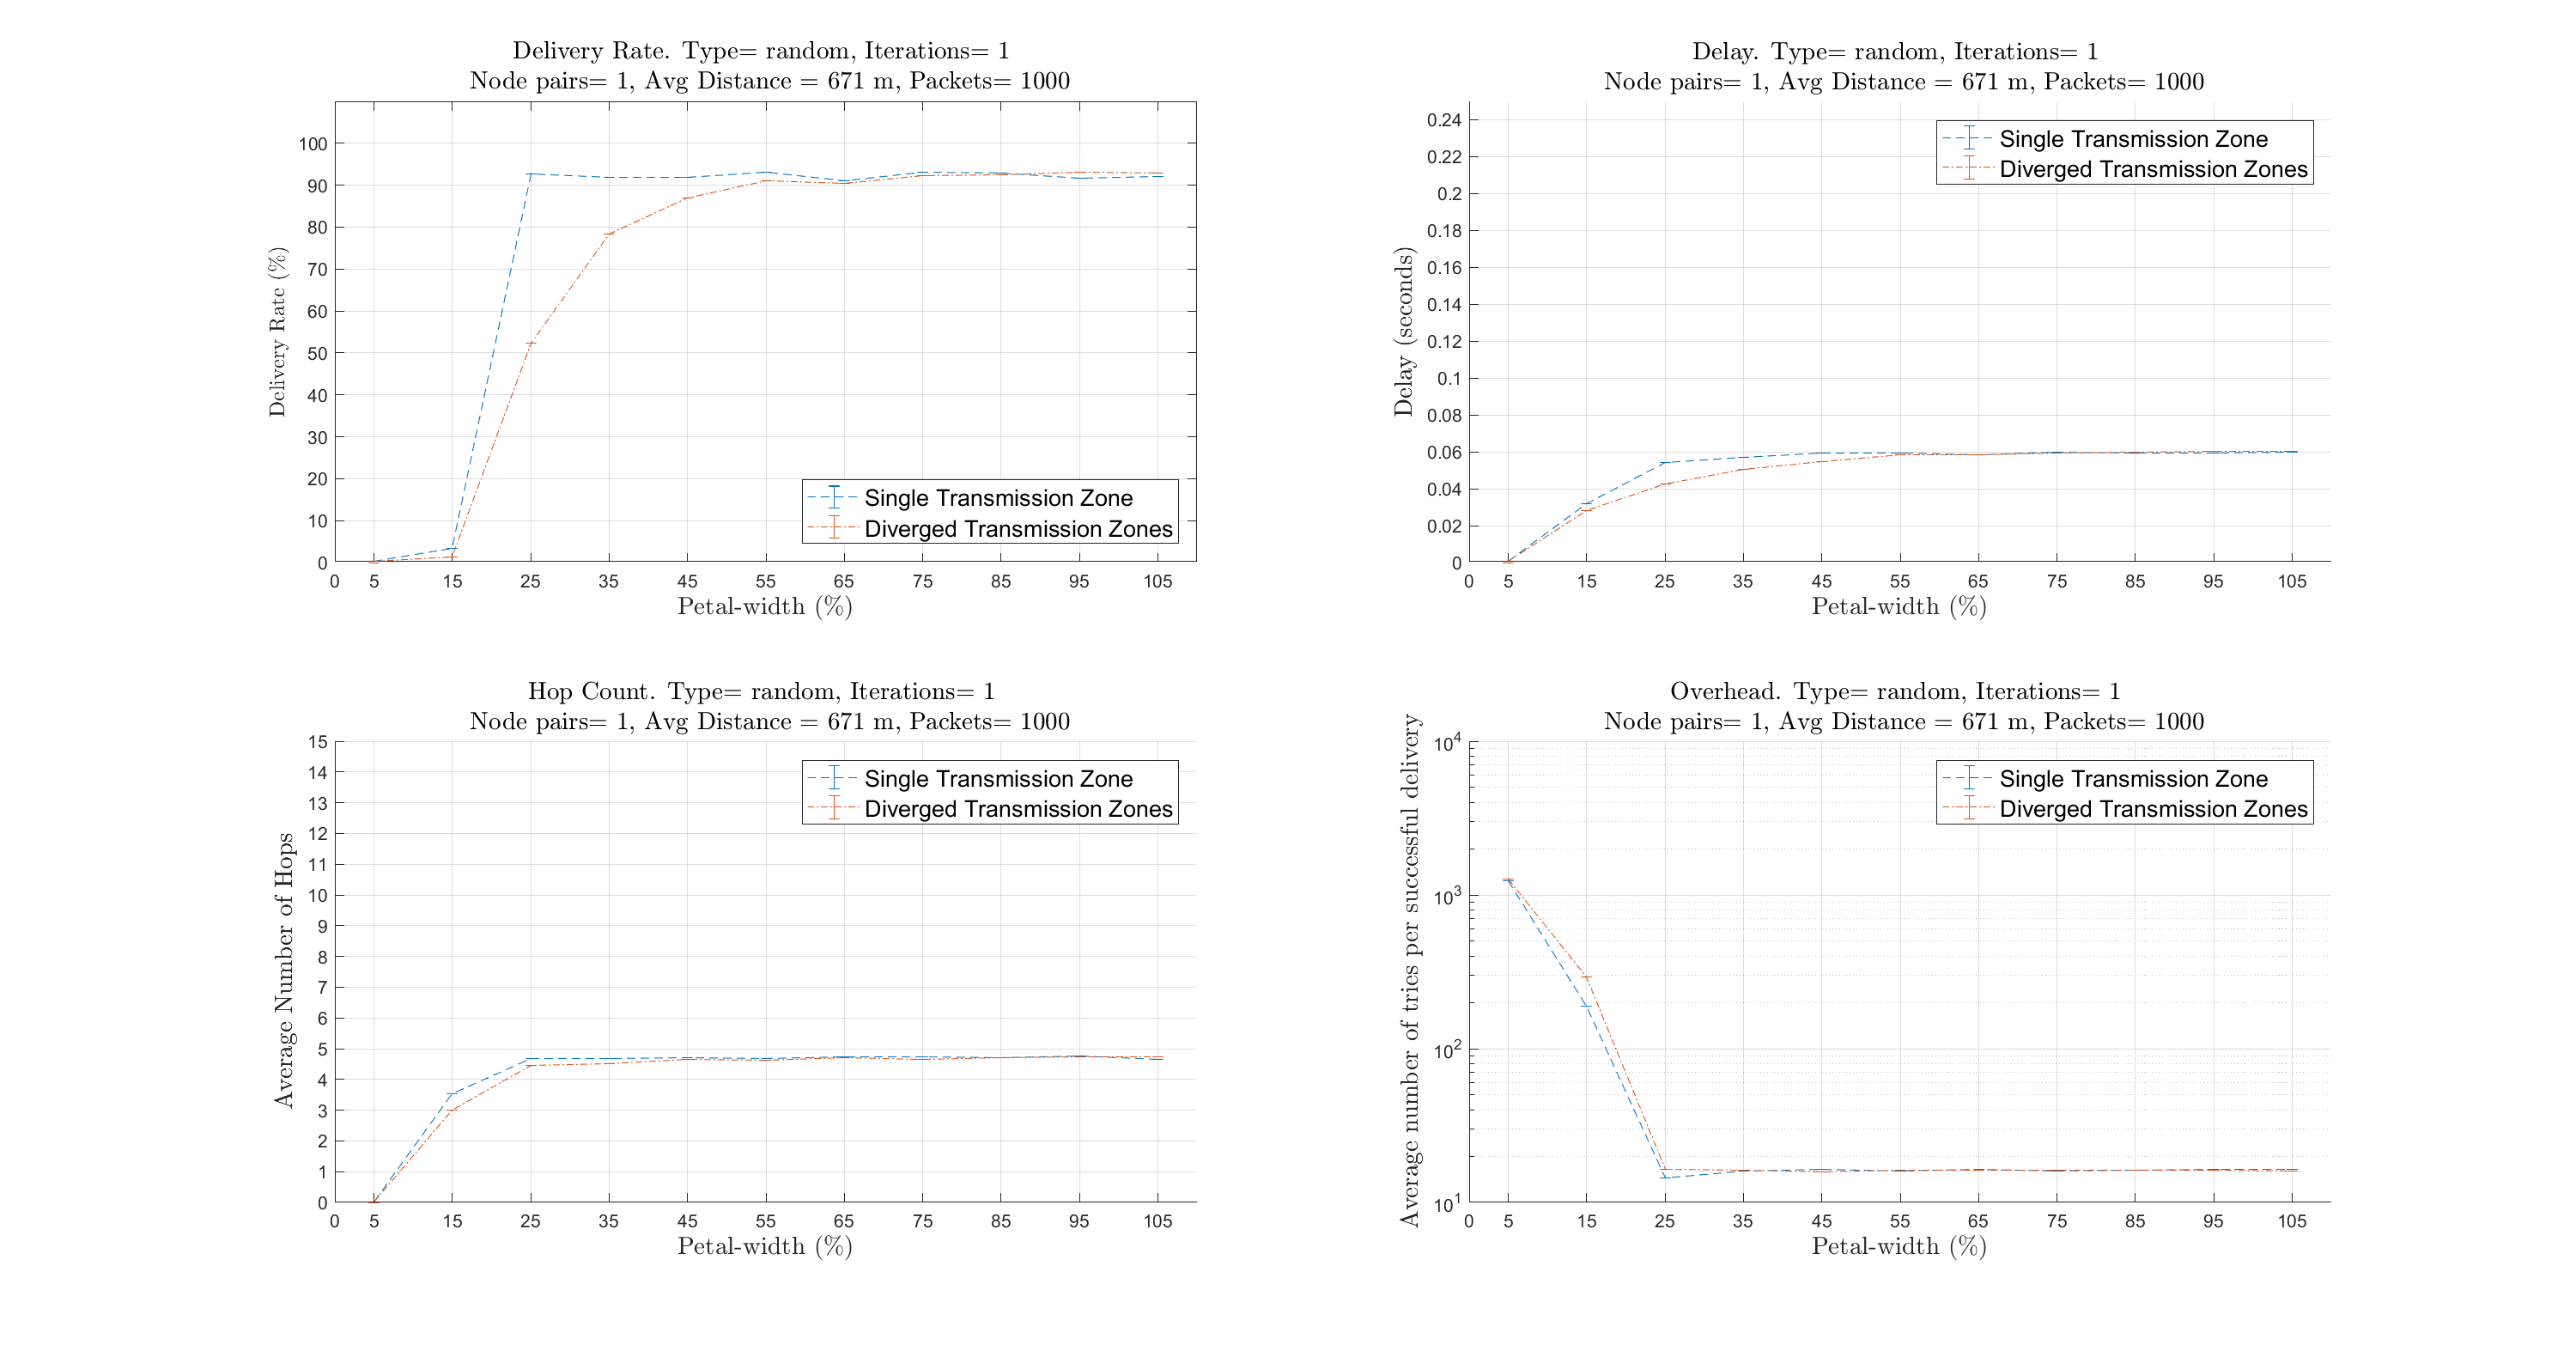
\includegraphics[width=1\textwidth]{ncsuthesis-0.6/Appendix-A/figs/petal_random.png}
\caption{Delivery ratio, end-to-end delay, hops and overhead for petal routing in a random distribution of UAVs.}
\label{fig:petal_random}
\end{figure}
\end{landscape}

\restoregeometry
\pagestyle{plain}
\thispagestyle{plain}
\newgeometry{margin=1in,lmargin=1.25in,footskip=\chapterfootskip, includehead, includefoot}

